\documentclass[man]{apa6}
\usepackage{lmodern}
\usepackage{amssymb,amsmath}
\usepackage{ifxetex,ifluatex}
\usepackage{fixltx2e} % provides \textsubscript
\ifnum 0\ifxetex 1\fi\ifluatex 1\fi=0 % if pdftex
  \usepackage[T1]{fontenc}
  \usepackage[utf8]{inputenc}
\else % if luatex or xelatex
  \ifxetex
    \usepackage{mathspec}
  \else
    \usepackage{fontspec}
  \fi
  \defaultfontfeatures{Ligatures=TeX,Scale=MatchLowercase}
\fi
% use upquote if available, for straight quotes in verbatim environments
\IfFileExists{upquote.sty}{\usepackage{upquote}}{}
% use microtype if available
\IfFileExists{microtype.sty}{%
\usepackage{microtype}
\UseMicrotypeSet[protrusion]{basicmath} % disable protrusion for tt fonts
}{}
\usepackage{hyperref}
\hypersetup{unicode=true,
            pdftitle={Does Music Convey Social Information to Infants?},
            pdfauthor={First Author~\& Ernst-August Doelle},
            pdfkeywords={keywords},
            pdfborder={0 0 0},
            breaklinks=true}
\urlstyle{same}  % don't use monospace font for urls
\usepackage{graphicx,grffile}
\makeatletter
\def\maxwidth{\ifdim\Gin@nat@width>\linewidth\linewidth\else\Gin@nat@width\fi}
\def\maxheight{\ifdim\Gin@nat@height>\textheight\textheight\else\Gin@nat@height\fi}
\makeatother
% Scale images if necessary, so that they will not overflow the page
% margins by default, and it is still possible to overwrite the defaults
% using explicit options in \includegraphics[width, height, ...]{}
\setkeys{Gin}{width=\maxwidth,height=\maxheight,keepaspectratio}
\IfFileExists{parskip.sty}{%
\usepackage{parskip}
}{% else
\setlength{\parindent}{0pt}
\setlength{\parskip}{6pt plus 2pt minus 1pt}
}
\setlength{\emergencystretch}{3em}  % prevent overfull lines
\providecommand{\tightlist}{%
  \setlength{\itemsep}{0pt}\setlength{\parskip}{0pt}}
\setcounter{secnumdepth}{0}
% Redefines (sub)paragraphs to behave more like sections
\ifx\paragraph\undefined\else
\let\oldparagraph\paragraph
\renewcommand{\paragraph}[1]{\oldparagraph{#1}\mbox{}}
\fi
\ifx\subparagraph\undefined\else
\let\oldsubparagraph\subparagraph
\renewcommand{\subparagraph}[1]{\oldsubparagraph{#1}\mbox{}}
\fi

%%% Use protect on footnotes to avoid problems with footnotes in titles
\let\rmarkdownfootnote\footnote%
\def\footnote{\protect\rmarkdownfootnote}


  \title{Does Music Convey Social Information to Infants?}
    \author{First Author\textsuperscript{1}~\& Ernst-August
Doelle\textsuperscript{1,2}}
    \date{}
  
\shorttitle{Title}
\affiliation{
\vspace{0.5cm}
\textsuperscript{1} Wilhelm-Wundt-University\\\textsuperscript{2} Konstanz Business School}
\keywords{keywords\newline\indent Word count: X}
\usepackage{csquotes}
\usepackage{upgreek}
\captionsetup{font=singlespacing,justification=justified}

\usepackage{longtable}
\usepackage{lscape}
\usepackage{multirow}
\usepackage{tabularx}
\usepackage[flushleft]{threeparttable}
\usepackage{threeparttablex}

\newenvironment{lltable}{\begin{landscape}\begin{center}\begin{ThreePartTable}}{\end{ThreePartTable}\end{center}\end{landscape}}

\makeatletter
\newcommand\LastLTentrywidth{1em}
\newlength\longtablewidth
\setlength{\longtablewidth}{1in}
\newcommand{\getlongtablewidth}{\begingroup \ifcsname LT@\roman{LT@tables}\endcsname \global\longtablewidth=0pt \renewcommand{\LT@entry}[2]{\global\advance\longtablewidth by ##2\relax\gdef\LastLTentrywidth{##2}}\@nameuse{LT@\roman{LT@tables}} \fi \endgroup}


\DeclareDelayedFloatFlavor{ThreePartTable}{table}
\DeclareDelayedFloatFlavor{lltable}{table}
\DeclareDelayedFloatFlavor*{longtable}{table}
\makeatletter
\renewcommand{\efloat@iwrite}[1]{\immediate\expandafter\protected@write\csname efloat@post#1\endcsname{}}
\makeatother
\usepackage{lineno}

\linenumbers

\authornote{Add complete departmental affiliations for each
author here. Each new line herein must be indented, like this line.

Enter author note here.

Correspondence concerning this article should be addressed to First
Author, Postal address. E-mail:
\href{mailto:my@email.com}{\nolinkurl{my@email.com}}}

\abstract{
One or two sentences providing a \textbf{basic introduction} to the
field, comprehensible to a scientist in any discipline.

Two to three sentences of \textbf{more detailed background},
comprehensible to scientists in related disciplines.

One sentence clearly stating the \textbf{general problem} being
addressed by this particular study.

One sentence summarizing the main result (with the words ``\textbf{here
we show}'' or their equivalent).

Two or three sentences explaining what the \textbf{main result} reveals
in direct comparison to what was thought to be the case previously, or
how the main result adds to previous knowledge.

One or two sentences to put the results into a more \textbf{general
context}.

Two or three sentences to provide a \textbf{broader perspective},
readily comprehensible to a scientist in any discipline.


}

\begin{document}
\maketitle

\section{Methods}\label{methods}

We report how we determined our sample size, all data exclusions (if
any), all manipulations, and all measures in the study.

\subsection{Participants}\label{participants}

\subsection{Material}\label{material}

\subsection{Procedure}\label{procedure}

\subsection{Data analysis}\label{data-analysis}

We used R (Version 3.5.2; R Core Team, 2018) and the R-packages
\emph{data.table} (Version 1.12.0; Dowle \& Srinivasan, 2019),
\emph{dplyr} (Version 0.8.0.1; Wickham, François, Henry, \& Müller,
2019), \emph{papaja} (Version 0.1.0.9842; Aust \& Barth, 2018),
\emph{pwr} (Version 1.2.2; Champely, 2018), and \emph{summarytools}
(Version 0.9.2; Comtois, 2019) for all our analyses.

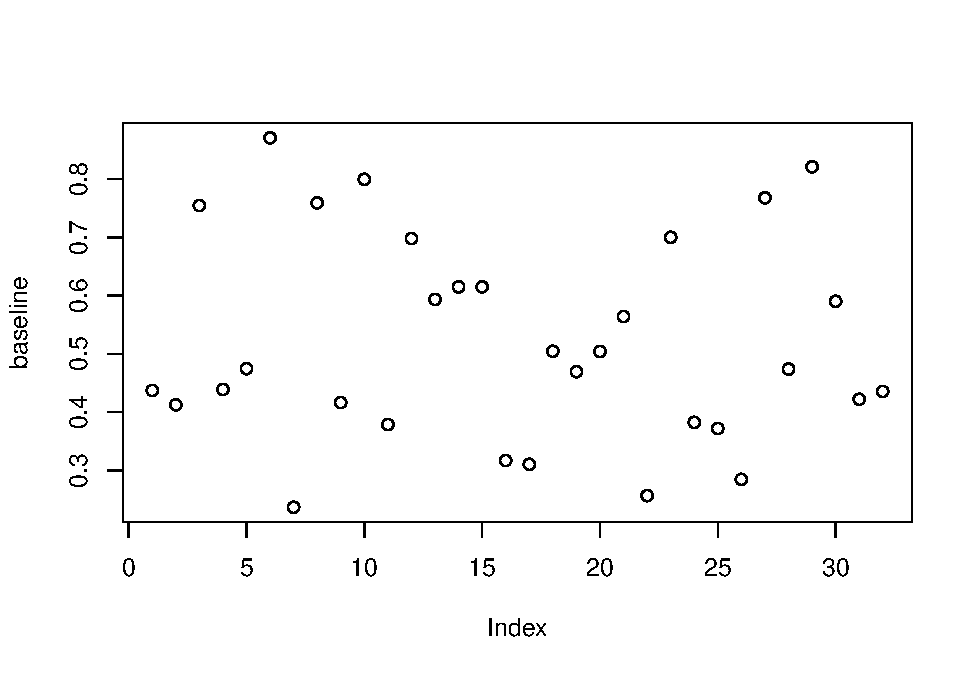
\includegraphics{Midterm_files/figure-latex/unnamed-chunk-5-1.pdf} \#
Results

\begin{verbatim}
## [1] 0.5210967
\end{verbatim}

\begin{verbatim}
## [1] 0.1769651
\end{verbatim}

\begin{verbatim}
## 
##  One Sample t-test
## 
## data:  baseline
## t = 0.67438, df = 31, p-value = 0.5051
## alternative hypothesis: true mean is not equal to 0.5
## 95 percent confidence interval:
##  0.4572940 0.5848994
## sample estimates:
## mean of x 
## 0.5210967
\end{verbatim}

\begin{verbatim}
## [1] 0.5210967
\end{verbatim}

\section{Discussion}\label{discussion}

\newpage

\section{References}\label{references}

\begingroup
\setlength{\parindent}{-0.5in} \setlength{\leftskip}{0.5in}

\hypertarget{refs}{}
\hypertarget{ref-R-papaja}{}
Aust, F., \& Barth, M. (2018). \emph{papaja: Create APA manuscripts with
R Markdown}. Retrieved from \url{https://github.com/crsh/papaja}

\hypertarget{ref-R-pwr}{}
Champely, S. (2018). \emph{Pwr: Basic functions for power analysis}.
Retrieved from \url{https://CRAN.R-project.org/package=pwr}

\hypertarget{ref-R-summarytools}{}
Comtois, D. (2019). \emph{Summarytools: Tools to quickly and neatly
summarize data}. Retrieved from
\url{https://CRAN.R-project.org/package=summarytools}

\hypertarget{ref-R-data.table}{}
Dowle, M., \& Srinivasan, A. (2019). \emph{Data.table: Extension of
`data.frame`}. Retrieved from
\url{https://CRAN.R-project.org/package=data.table}

\hypertarget{ref-R-base}{}
R Core Team. (2018). \emph{R: A language and environment for statistical
computing}. Vienna, Austria: R Foundation for Statistical Computing.
Retrieved from \url{https://www.R-project.org/}

\hypertarget{ref-R-dplyr}{}
Wickham, H., François, R., Henry, L., \& Müller, K. (2019). \emph{Dplyr:
A grammar of data manipulation}. Retrieved from
\url{https://CRAN.R-project.org/package=dplyr}

\endgroup


\end{document}
